%! Author = admin
%! Date = 14.12.2022

% Preamble
\documentclass[a4paper,12pt]{article}

% Packages
\usepackage{multirow}
\usepackage{wrapfig}
\usepackage[T2A]{fontenc}
\usepackage[utf8]{inputenc}
\usepackage[english,russian]{babel}
\usepackage{indentfirst}
\usepackage[usenames]{color}
\usepackage[a4paper,top=0.9cm,bottom=0.9cm,left=0.75cm,right=0.75cm,marginparwidth=0.75cm]{geometry}
\usepackage{colortbl}
\usepackage{graphicx}%Вставка картинок правильная
\usepackage{float}%"Плавающие" картинки
\usepackage{wrapfig}
\usepackage{hyperref}
\usepackage{subcaption}
\usepackage[rgb]{xcolor}
\usepackage{todonotes}
\usepackage{amsmath,amsfonts,amssymb,amsthm,mathtools}
\usepackage{makecell}


% package to open file containing variables
\usepackage{datatool, filecontents}
\usepackage{colortbl}
\usepackage{booktabs}
\DTLsetseparator{,}% Set the separator between the columns.

% import data
\DTLloadrawdb[noheader, keys={thekey,thevalue}]{output_data}{C:/labas/1.4.1/data/output_data.csv}
% Loads output_data.csv with column headers 'thekey' and 'thevalue'
\newcommand{\var}[1]{\DTLfetch{output_data}{thekey}{#1}{thevalue}}

% Document
\begin{document}
    \begin{centering}
        \section* {{\fboxsep=0pt\colorbox{green!50}{\strut Обработка данных:}}}
    \end{centering}

    \begin{table}[h!]
        \centering
        \begin{tabular}{|c|c|c|c|c|c|c|c|c|}
            \hline
            $a$, мм & 470 & 430 & 390 & 340 & 300 & 250 & 200 & 150 \\ \hline
            $\varepsilon_{a}$ & \var{reA1} & \var{reA2} & \var{reA3} & \var{reA4} & \var{reA5} & \var{reA6} &
            \var{reA7} & \var{reA8}\\ \hline
            $x_{\text{ц}}$, мм & 432 & 395 & 358 & 311 & 275 & 230 & 183 & 137
            \\ \hline
            $\varepsilon_{x_{\text{ц}}}$ & \var{reX1} & \var{reX2} & \var{reX3} & \var{reX4} & \var{reX5} & \var{reX6} &
            \var{reX7} & \var{reX8}\\ \hline
            $t$, c & \var{t1} & \var{t2} & \var{t3} & \var{t4} & \var{t5} & \var{t6} & \var{t7} & \var{t8}
            \\ \hline
            $\sigma_{t}$, c & \var{fet1} & \var{fet2} & \var{fet3} & \var{fet4} & \var{fet5} & \var{fet6} &
            \var{fet7} & \var{fet8} \\ \hline
            $\varepsilon_{t}$ & \var{ret1} & \var{ret2} & \var{ret3} & \var{ret4} & \var{ret5} & \var{ret6} &
            \var{ret7} & \var{ret8}
            \\ \hline
            $T$, c & \var{T1} & \var{T2} & \var{T3} & \var{T4} & \var{T5} & \var{T6} & \var{T7} & \var{T8}
            \\ \hline
            $\sigma_{T}$, c & \var{feT1} & \var{feT2} & \var{feT3} & \var{feT4} & \var{feT5} & \var{feT6} &
            \var{feT7} & \var{feT8} \\ \hline
            $\varepsilon_{T}$ & \var{reT1} & \var{reT2} & \var{reT3} & \var{reT4} & \var{reT5} & \var{reT6} &
            \var{reT7} & \var{reT8}
            \\ \hline
            $g$, м/с^2 & \var{G1} & \var{G2} & \var{G3} & \var{G4} & \var{G5} & \var{G6} & \var{G7} & \var{G8}
            \\ \hline
            $\sigma_{g}$, м/с^2 & \var{Ger1} & \var{Ger2} & \var{Ger3} & \var{Ger4} & \var{Ger5} & \var{Ger6} &
            \var{Ger7} & \var{Ger8} \\ \hline

        \end{tabular}
        \caption{Вычисление ускорения свободного падения по формуле (1)}
    \end{table}

    Теперь по этим результатам вычислим среднее ускорение свободного падения:
    $$g = \frac{4\pi ^2}{T^2} \cdot \frac{\frac{l^2}{12}+a^2}{(1+\frac{m_{\text{пр}}}{m_{\text{ст}}})x_{\text{цм}}} $$ $$g = \var{Gav} \pm 0.110  \text{м}/\text{с}^2$$

    \begin{figure}[h!!]
        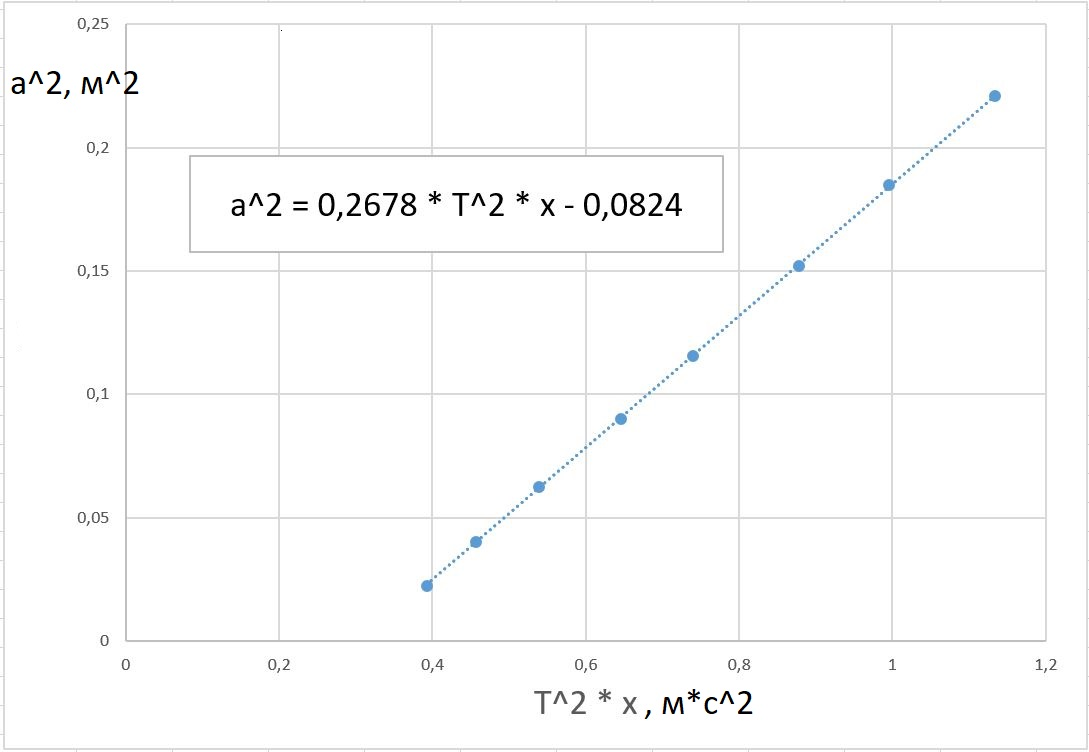
\includegraphics{Capture}
        \caption{Линейная зависимость, иллюстрирующая формулу (3)}
    \end{figure}

    Исходя из метода наименьших квадратов: $k$ = 0.2678, значит, по формуле (4), $g$ = 9.701 м/с^2



\end{document}